\chapter{Fundamentos de la Inteligencia Artificial y sus herramientas}\chaptermark{Fundamentos de la IA y herramientas}

	\section{Convolución y correlación cruzada}
	
		Una de las operaciones matemáticas más conocidas y que es más usada al trabajar con señales e imágenes es la llamada convolución, denotada por $\ast$, y dadas las funciones $f(t)$ y $g(t)$, su convolución se define de la siguiente manera. 
		
		$$
		(f \ast g)(t) = \int_{-\infty}^\infty f(\tau)g(t - \tau) d\tau
		$$
		
		En este caso se está asumiendo que el dominio de $f(\tau)g(t - \tau)$ es $\mathbb{R}$, lo que permite integrar sobre todo $\mathbb{R}$, de lo contrario, se modifica la definición para integrar solo sobre un intervalo $[a, b]$. En general, esta operación crea una nueva función a partir de otras dos, que indica cómo interactúan entre sí, y que permite aplicar filtros a señales e imágenes. Como se acaba de comentar para el caso de las imágenes, se puede tratar con señales que no dependan únicamente de una variable, pues estas se representan como una función de dos variables $f(u, v)$. En este caso, la convolución queda definida de la siguiente manera. 
		
		$$
		(f \ast g)(u, v) = \int_{-\infty}^\infty\int_{-\infty}^\infty f(\xi, \eta)g(u - \xi, v - \eta) d\xi d\eta
		$$
		
		Partiendo de las primera definición mostrada, se pueden demostrar algunas propiedades útiles que cumple la convolución: 
		
		\begin{itemize}
			\item Conmutativa: $f \ast g = g \ast f$
			\item Asociativa: $f \ast (g \ast h) = (f \ast g) \ast h$
			\item Distributiva: $f \ast (g + h) = (f \ast g) + (f \ast h)$
			\item Derivada: $\frac{d}{dt}(f \ast g) = \frac{df}{dt}\ast g = \frac{dg}{dt}\ast f$
			\item Teorema de convolución: $\mathscr{L}\{f \ast g\} = \mathscr{L}\{f\} \cdot \mathscr{L}\{g\}$
		\end{itemize}
		
		Si bien en las definiciones previas se ha tomado la integral y tanto $\mathbb{R}$ como $\mathbb{R}^2$ como dominios continuos sobre los que calcular la convolución, no se debe olvidar que las imágenes no dejan de ser matrices o funciones de dos variables con un dominio discreto, por lo que se debe presentar una definición adecuada a este caso. 
		
		$$
		(f \ast g)(u, v) = \sum_{i=-k}^{k}\sum_{j=-k}^{k} g(i, j)f(u - i, v - j)
		$$
		
		En la expresión anterior, a la función $g(u, v)$ se le llama filtro o \textit{kernel} de convolución. A continuación se muestra un ejemplo de cómo calcular una convolución. 
		
		$$
		\begin{gathered}
			\begin{pmatrix}
				\tikzmarknode{a1}{1}& 2& 3& 4& 5\\ 
				5& 6& 7& 8& 9\\ 
				9& 8& \tikzmarknode{a2}{7}& 6& 5\\ 
				5& 4& 3& 2& 1\\
				1& 2& 3& 4& 5
			\end{pmatrix}
			\ast
			\begin{pmatrix}
				\tikzmarknode{b1}{1} & 0 & 0\\
				0 & 1 & 0\\
				0 & 0 & \tikzmarknode{b2}{1}
			\end{pmatrix}
			=
			\begin{pmatrix}
				\tikzmarknode{c1}{14} & 15 & 16\\
				16 & 15 & 14\\
				16 & 15 & 14
			\end{pmatrix}\\
			1 \cdot 1 + 2 \cdot 0 + 3 \cdot 0 + 5 \cdot 0 + 6 \cdot 1 + 7 \cdot 0 + 9 \cdot 0 + 8 \cdot 0 + 7 \cdot 1 = 14\\
			2 \cdot 1 + 3 \cdot 0 + 4 \cdot 0 + 6 \cdot 0 + 7 \cdot 1 + 8\cdot 0 + 8\cdot 0 + 7 \cdot 0 + 6 \cdot 1 = 15\\
			\vdots\\
			7 \cdot 1 + 6 \cdot 0 + 5 \cdot 0 + 3 \cdot 0 + 2 \cdot 1 + 1 \cdot 0 + 3 \cdot 0 + 4 \cdot 0 + 5 \cdot 1 = 14
		\end{gathered}
		\begin{tikzpicture}[remember picture, overlay]
			\draw ([shift={(-.5mm, .5mm)}]a1.north west) rectangle ([shift={(.5mm, -.5mm)}]a2.south east);
			\draw ([shift={(-.5mm, .5mm)}]b1.north west) rectangle ([shift={(.5mm, -.5mm)}]b2.south east);
			\path[->] ([shift={(-.5mm, .5mm)}]a1.north) edge [bend left = 15] ([shift={(-.5mm, 1mm)}]c1.north);
			\path[->] ([shift={(-.5mm, .5mm)}]b1.north) edge [bend left = 20] ([shift={(-.5mm, 1mm)}]c1.north);
		\end{tikzpicture}
		$$
		
		Aplicando diferentes kernels de convolución a una imagen se pueden extraer diferentes tipos de características de una imagen, como por ejemplo bordes. El filtro Sobel es capaz de hacer esto con los kernels que se muestran a continuación, pues se comportan como aproximaciones de las derivadas parciales de la imagen en un punto teniendo en cuenta los píxeles cercanos. 
		
		\begin{align*}
			G_u &= \frac{\partial f(u, v)}{\partial u} \approx \begin{pmatrix}
				-1 & 0 & 1\\
				-2 & 0 & 2\\
				-1 & 0 & 1
			\end{pmatrix}&
			G_v &= \frac{\partial f(u, v)}{\partial v} \approx \begin{pmatrix}
				-1 & -2 & -1\\
				0 & 0 & 0\\
				1 & 2 & 1
			\end{pmatrix}
		\end{align*}
		
		\begin{figure}[!h]
			\centering
			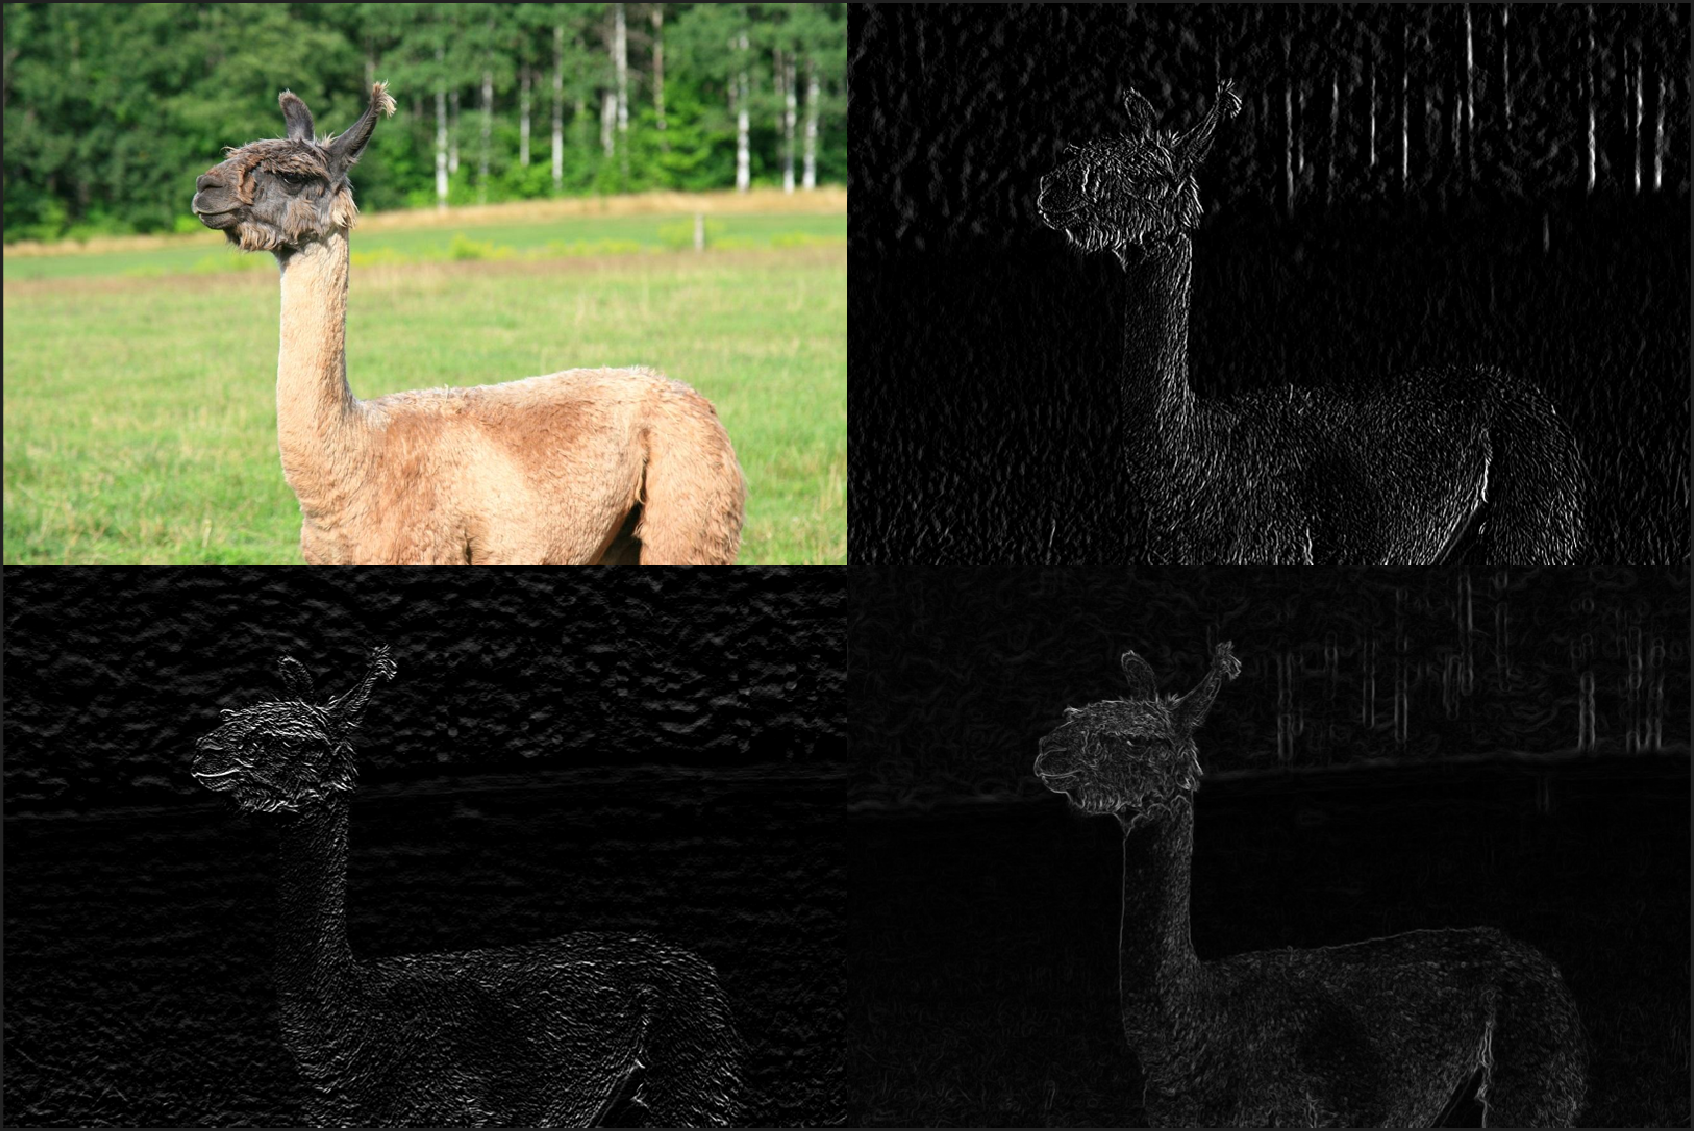
\includegraphics[scale = .4]{ejemplo_sobel}
			\caption{Detección de bordes aplicando los kernel Sobel}
			\label{fig:sobel}
		\end{figure}
		
		A continuación se va a calcular la convolución de la matriz del ejemplo anterior con $G_u$. Para comprobar los cálculos, se puede realizar esto con la función \texttt{convn} de MATLAB. Al realizar los cálculos a mano tal y como se ha mostrado en el ejemplo anterior, se obtiene como resultado la matriz $A$, mientras que MATLAB devuelve la matriz $B$ como resultado de \texttt{convn(X, $G_u$, 'valid')}. ¿Qué acaba de suceder? ¿Está mal codificada la función de MATLAB? ¿Está mal realizado el ejemplo?
		
		\begin{align*} A &= 
			\begin{pmatrix}
				4 & 4 & 4\\
				-4 & -4 & -4\\
				-4 & -4 & -4
			\end{pmatrix}&
			B &= \begin{pmatrix}
				-4 & -4 & -4\\
				4 & 4 & 4\\
				4 & 4 & 4
				\end{pmatrix}
		\end{align*}
		
		La respuesta a estas preguntas se podría resumir en que se ha realizado una ``pequeña trampa'' a la hora de calcular la convolución manualmente en el ejemplo, ya que no se ha aplicado correctamente la definición dada. ¿Qué sentido tiene hacer esto? En visión artificial y tratamiento de imágenes, muchos autores y librerías llaman convolución a la operación que se ha mostrado en el primer ejemplo, cuando en realidad no lo es y trae lugar a confusión. Dicha operación se llama correlación cruzada, denotada por $(\star)$, y que es muy similar a la convolución, pues su principal diferencia es que en la convolución ``real'', el kernel se rota 180 grados antes de calcular la convolución ``falsa'' o correlación cruzada, es decir, $X \ast Y = X \star (R_{180} \cdot Y)$. La correlación cruzada de dos imágenes (matrices) se define de la siguiente manera. 
		
		$$
		(f \star g)(u, v) = \sum_{i=-k}^{k}\sum_{j=-k}^{k} g(i, j)f(u + i, v + j)
		$$
		
		Esta operación sí es con la que realmente se aplican los filtros a las imágenes y con la que se trabaja en general en el campo de la visión artificial. Es importante ver que ahora, al contrario que con la convolución, $f \star g \neq g \star f$. Algunas librerías de visión artificial tratan a la correlación cruzada como convolución debido al frecuente uso que tiene una sobre la otra y la forma similar que tienen de calcularse. Un ejemplo es OpenCV en la documentación de su función \texttt{filter2D}, donde se comenta que aplica una convolución cuando realmente aplica la correlación cruzada. Finalmente, como se verá en próximos capítulos, las famosas redes neuronales convolucionales, no aplican convoluciones sino correlaciones cruzadas. 